\section{POODLE}

\subsection{a) Verschaffen Sie sich Zugang zur PHP SessionID des anzugreifenden Clients. Dokumentieren Sie dabei alle Zwischenschritte.}
Im ersten Fenster wird der HTTPS-Server gestartet und die Server-IP übergeben. Dieser Server fungiert stellvertretend für einen XSS-Angriff. Dieser läuft nun und ist über die Angreifer-IP 192.168.2.5 erreichbar. Er sendet an den Server 192.168.2.200.

In einem zweiten Fenster wird der MIT-Attack gestartet (\autoref{fig:mitm}). Mittels ARP-Poisoning werden sämtliche Anfragen unseres Netzes an uns selbst weitergeleitet. Das Skript wird gestartet. Den bettercap-Anweisungen folgend wird das Poisoning durchgeführt. Will nun das Opfer auf den Server, wird er an den Angreifer weitergeleitet.
\begin{figure}[H]
    \centering
    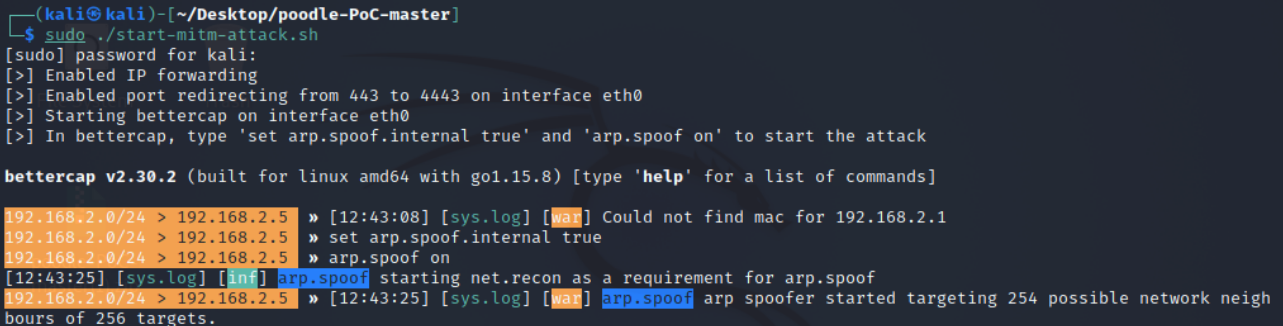
\includegraphics[width=1\linewidth]{start-mitm-attack.png}
    \caption{start-mitm-attack.sh}
    \label{fig:mitm}
\end{figure}
\noindent In einem dritten Fenster wird der eigentliche Poodle-Exploid gestartet (\autoref{fig:poodle-start}). Dazu wird zunächst die Angreifer-IP und die Server-IP übergeben, jeweils mitsamt den dazugehörigen Ports. Außerdem werden die Blöcke übergeben, in denen die Session-ID zu finden sein wird.
\begin{figure}[H]
    \centering
    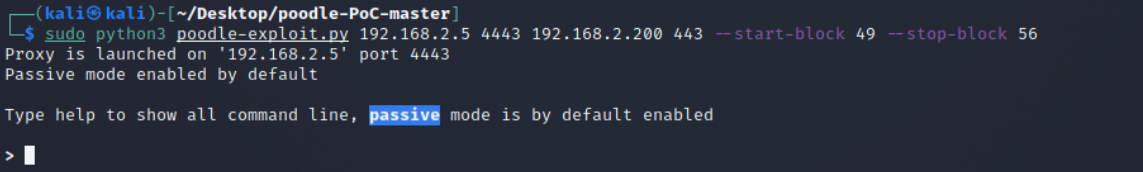
\includegraphics[width=1\linewidth]{poodle-exploid.png}
    \caption{poodle-exploit.py}
    \label{fig:poodle-start}
\end{figure}
\noindent Als nächstes loggt sich das Opfer im Server ein. (\autoref{fig:signin}).
\begin{figure}[H]
    \centering
    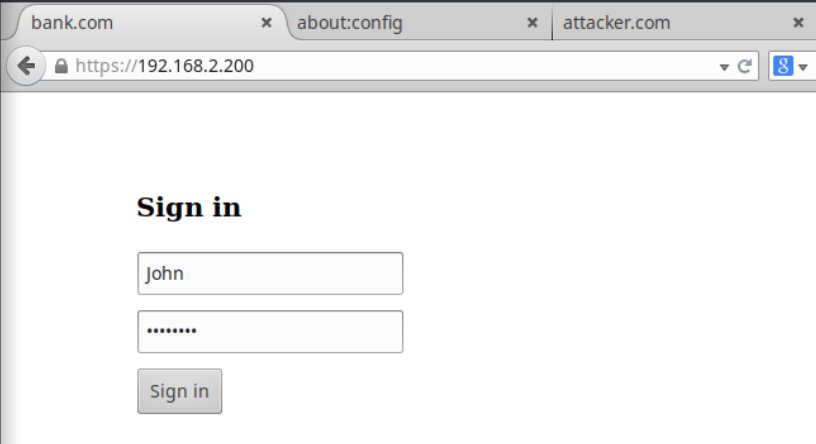
\includegraphics[width=0.5\linewidth]{signin.png}
    \caption{sign in: John:mypasswd}
    \label{fig:signin}
\end{figure}
\noindent In dem Browser der Opfers kann verifiziert werden, dass die veraltete TLS-Version verwendet wird. Das ist in \autoref{fig:aboutconfig} zu sehen.
\begin{figure}[H]
    \centering
    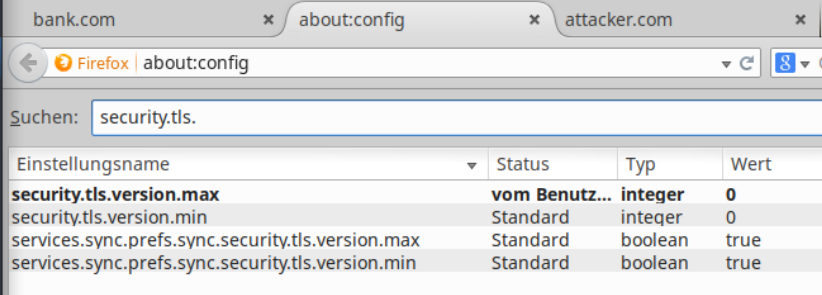
\includegraphics[width=0.5\linewidth]{aboutconfig.png}
    \caption{about:config}
    \label{fig:aboutconfig}
\end{figure}
\noindent Nachdem alles vorbereitet ist, kann der Angriff gestartet werden. Die nachfolgenden Schritte sind in \autoref{fig:ragebait} graphisch dokumentiert. Der Angreifer startet die downgrade-Attacke über das poodle-exploit-Skript. Dazu gibt er das Schlüsselwort \enquote{downgrade} ein. Im nächsten Schritt muss das Skript die Blocklength herausfinden. Dies passiert im \textttt{search} Modus. Wärend dieser Modus aktiv ist, kann mit einem klick auf der Seitet des Angreifers die Blocklänge bestimmt werden. Nachden die Blocklänge bestimmt wurde kann der \textttt{active} Mode gestartet werden. In diesem Modus passiert dann die Entschlüsselung. Mit einem Klick auf der Seite des Angreifers wird dann der Angriff gestartet und die PHP-SessionId nach und nach entschlüsselt.
\begin{figure}[H]
    \centering
    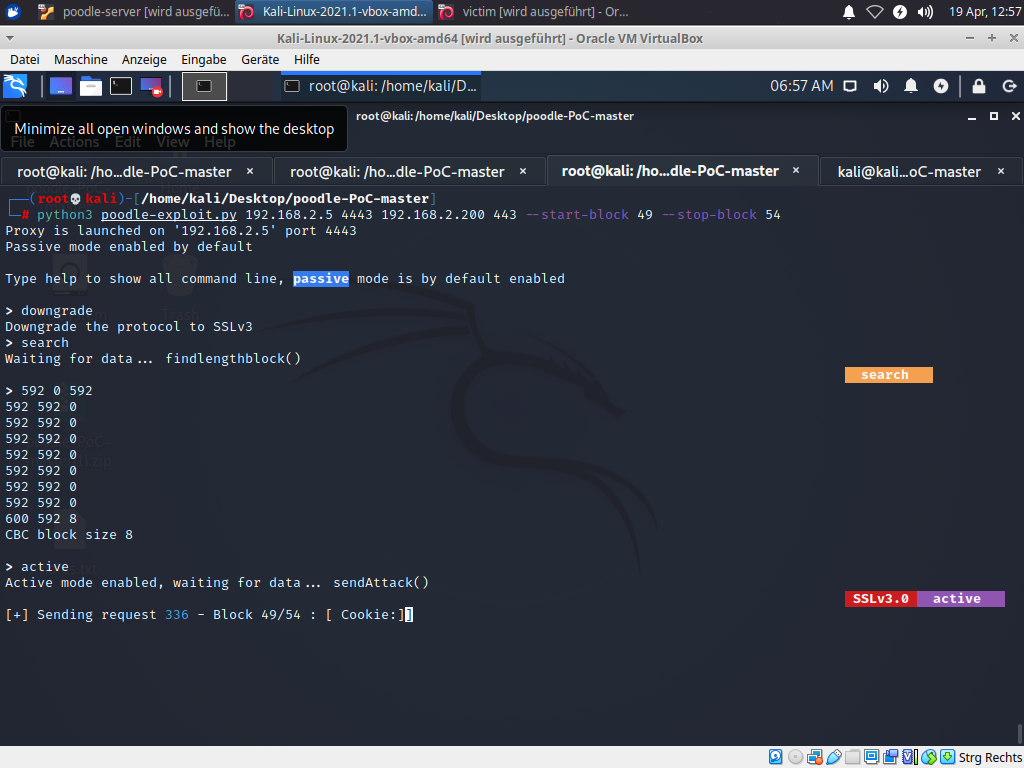
\includegraphics[width=0.75\linewidth]{ragebait.png.png}
    \caption{POODLE-Angriff}
    \label{fig:ragebait}
\end{figure}
\noindent Nachdem das Skript beendet wurde wird die gefundene Session-ID ausgegeben. Diese ist in \autoref{fig:success} zu erkennen.
\begin{figure}[H]
    \centering
    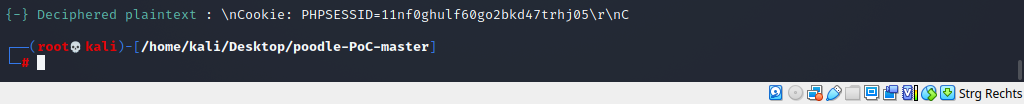
\includegraphics[width=0.75\linewidth]{success.png}
    \caption{Session-ID Gefunden}
    \label{fig:success}
\end{figure}

\subsection{b) Erklären Sie die Funktionsweise des Angriffs. Der Fokus liegt dabei auf dem Poodle Angriff selbst und nicht der Vorbereitung wie dem MitM. Hierfür sollte das Dokument eine ausreichend detaillierte Hilfe bieten. Gleichfalls können Sie ja auch alle Schritte selbst analysieren, bspw. via Wireshark, über die Webbrowser Konsole oder über die Ausgabe der einzelnen Schritte des Python Angriffskriptes selbst.}
Der Angriff ist eine Kombination aus einer Downgrade-Attacke und einem Padding-Orakel-Angriff. Zunächst einmal muss per Downgrade-Attacke die zwischen Client und Server genutzte SSL-Version auf 3.0 heruntergehandelt werden. Dies ist essenziell, da diese Version u.a. die Padding-Blöcke nicht alle auf ihre Korrektheit überprüft. Dadurch wird ein Padding-Orakel-Angriff erst ermöglicht. Das letzte Byte des Paddings gibt dabei die Länge des Paddings an. Außerdem muss der DES im CBC Mode verwendet werden. Die Verschlüsselung fungiert also gilt für die Entschlüsselung:
$$
DES_{dec}(c_i[k]) \oplus c_{i-1}[k] = p_i[k]
\text{, mit $i$ als Blockposition und $k$ als Byte-Position}
$$
Der Angreifer sorgt dafür, dass der Nutzer eine Nachricht schickt, deren Inhalt exakt so groß ist, dass der letzte Verschlüsselungsblock vollständig aus Padding-Bytes besteht. Bei einer Blockbröße von 8 Byte weiß er daher, dass der Wert des letzten Bytes 0x07 sein muss bzw. dass der Server nur Nachrichten akzeptieren wird, deren letztes Padding-Byte entschlüsselt 0x07 ergibt, da andernfalls der HMAC inkorrekt ist.

Nun vollführt der Angreifer den Padding-Orakel-Angriff. An die Stelle des Padding-Blocks setzt er denjenigen Block, der den Cookie enthält und sendet die Nachricht an den Server. Nimmt der Server die Nachricht an, weiß der Angreifer, welchen Wert das letzte Byte des Cookie-Blocks entschlüsselt hat, nämlich 0x07. Wird die Nachricht nicht angenommen, bricht die Verbindung zum Server ab und ein neuer Handshake mit neuem Key wird vollzogen, wodurch eine erneute Chance auf ein korrektes Ergebnis besteht. Bei Erfolg besitzt der Angreifer folgende Information:
$$
\begin{align}
DES_{dec}(c_n[7]) \oplus c_{n-1}[7] &= 0x07 \\
\end{align}
$$
Ferner weiß der Angreifer, dass der Block $n$ in Wahrheit dem Cookie-Block $i$ entspricht. Es gilt also:
$$
DES_{dec}(c_n[7]) = DES_{dec}(c_i[7]) = P_i[7] \oplus c_{i-1}[7]
$$
Kombiniert der Angreifer diese beiden Gleichungen, ergibt sich:
$$
(p_i[7] \oplus c_{i-1}[7]) \oplus c_{n-1}[7] = 0x07
$$
und ferner nach Umstellung:
$$
p_i[7] = c_{i-1}[7] \oplus c_{n-1}[7] \oplus 0x07
$$
Der Angreifer ist nun in der Lage, das niederwertigste Byte des Cookie-Blocks zu berechnen. Jetzt verschiebt der Angreifer die Nachricht um ein Byte, sodass das neue niederwertigste Byte dem nächsten-höheren Byte des Cookie-Blocks entspricht, indem er der Pfad-Anfrage ein Byte anhängt und vom HTTP-Body ein Byte entfernt. Die Prozedur wird wiederholt. So entschlüsselt der Angreifer nach und nach den gesamten Block und kommt an die Session-ID. 

\subsection{c) Lässt sich dieser Angriff heute noch durchführen und wenn nein, was verhindert heute diesen Angriff (Bezug auf die Teilkomponenten nehmen)?}
Heute ist dieser Angriff kaum noch möglich, da er die SSL-Version 3.0 voraussetzt und diese seit 2014 als unsicher gilt ist. Die allermeisten (modernen) Server unterstützen bzw. verbieten daher diese Version. Allerdings funktioniert dieser Angriff immer noch auf gewissen alten Systemen, die SSL 3.0 immer noch verwenden und bei fehlerhaften Implementierungen. Außerdem verhindert bzw. erschwert die Same-Origin-Policy XSS-Attacks, was fatal für den Angriff ist.